\mychapter{vision}{Vision, concepts and principles}
\begin{figure}
  \begin{center}
    \centerline{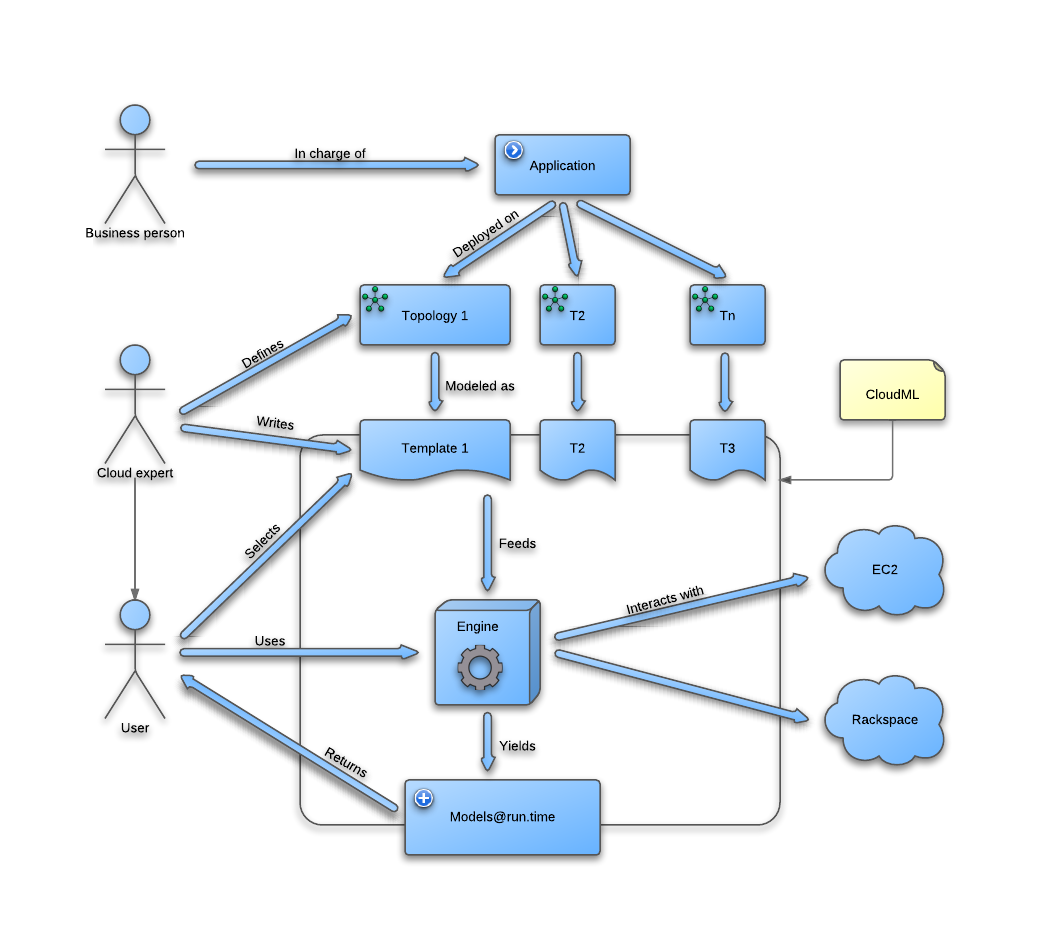
\includegraphics[width=1.5\linewidth]{img/big-picture.png}}
    \caption{``Big picture'', overview of CloudML procedure flow.}
    \label{fig:big-picture}
  \end{center}
\end{figure}


In this chapter the core idea of CloudML will be presented,
how a procedure of node provisioning is conducted in the perspective of different actors.

The concept and principle of CloudML is to be an easier and more reliable
path into cloud computing for IT-driven businesses of variable sizes.
The tool is visioned to parse and execute template files representing topologies
of instances in the cloud. 

\section{The ``big picture''}

The vision of CloudML is reflected through \citefig{big-picture} which gives
an overview of the procedure flow in and around CloudML.

\paragraph{Domain of CloudML.}

Inside \citefig{big-picture} there is an area pointed out as \emph{CloudML},
this area contain components necessary to implement in order to fulfill
the vision as a whole.
Every part within the designated area is some physical aspect in the 
implementation, and therefore core parts of the contribution.

\paragraph{The actors.}

In \citefig{big-picture} there are three actors,
\begin{ii}
  \iitem business person representing someone with administrative or manager position which
    defines and controls demands for application functionality and capabilities.
    The next actor,
  \iitem cloud expert has a greater knowledge of the cloud domain \eg Cloud providers,
    services these offer, limitations, API support and prices.
    The last actor,
  \iitem user is a person which directly utilize CloudML to do provisioning.
    This physical person may or may not have the role of cloud expert, hence 
    the actor extends from cloud expert.
\end{ii}

\paragraph{Application and topologies.}

The business person is in charge of the application, he or she has a need
for an application that can fulfill certain tasks, and to do handle these 
tasks reflecting demands are made.
The cloud expert use the requirements sketched by the business person to 
define and design node topologies which tackles the application demands.
A topology is a map of nodes connected together in a specific pattern, 
defined by the cloud expert.
In a topology there is also information about node attributes 
\eg \myac{CPU} power and \myac{RAM} sizes.
He or she might create several topologies to fulfill the application demands.

\paragraph{Templates.}

The next step is to create templates based on the topologies, this is done by
the cloud expert.
A template is a digital reflection of a topology including the attributes and some additional 
information such as node names and template labeling.
It is also possible to define more than one topology within a single template,
but for the sake of tidiness, clarity and technical limitations it 
should not be possible to define cross-provider (\emph{multicloud}) nodes in a single topology.
This itself does not mean CloudML will not support multicloud provisioning,
instead such functionality is achieved by utilizing more than one template,
which will not retain a full multicloud deployment.

\paragraph{Engine.}

When the cloud expert have designed and created the necessary templates the next actor, 
user, will continue the procedure.
The user select the templates and feed them into the engine.
The engine is the core of the implementation handling several steps and executing
most of the CloudML logic.
The engine operates in five different steps, \
\begin{ii}
  \iitem convert the template files into a native format for later use, 
  \iitem convert pure nodes into instances ready for provisioning, 
  \iitem connect to all the desired providers and 
  \iitem propagate these. Lastly it will produce
  \iitem models@run.time of the nodes being propagated.
\end{ii}
